%%%%%%%%%%%%%%%%%%%%%%%%%%%%%%%%%%%%%%%%%%%%%%%%%%%%%%%%%%%%%%%%%%%%%%%%%%%%%%%%%%
\begin{frame}[fragile]\frametitle{}
\begin{center}
{\Large Conclusions}
\end{center}
\end{frame}

%%%%%%%%%%%%%%%%%%%%%%%%%%%%%%%%%%%%%%%%%%%%%%%%%%%%%%%%%%%
\begin{frame}[fragile]\frametitle{ChatGPT Ultimate Prompting Guide}

\begin{itemize}
\item Tone: Specify the desired tone (e.g., formal, casual, informative, persuasive).
\item Format: Define the format or structure (e.g., essay, bullet points, outline, dialogue). 
\item Act as: Indicate a role or perspective to adopt (e.g., expert, critic, enthusiast). 
\item Objective: State the goal or purpose of the response (e.g., inform, persuade, entertain). 
\item Context: Provide background information, data, or context for accurate content generation. 
\item Scope: Define the scope or range of the topic.
\item Keywords: List important keywords or phrases to be included.
\item Limitations: Specify constraints, such as word or character count.
\item Examples: Provide examples of desired style, structure, or content.
\item Deadline: Mention deadlines or time frames for time-sensitive responses. 
\end{itemize}	 


{\tiny (Ref: LinkedIn post by Generative AI, Twitter by Aadit Sheth, Source : Reddit)}
			

\end{frame}


%%%%%%%%%%%%%%%%%%%%%%%%%%%%%%%%%%%%%%%%%%%%%%%%%%%%%%%%%%%
\begin{frame}[fragile]\frametitle{ChatGPT Ultimate Prompting Guide}

\begin{itemize}
\item Audience: Specify the target audience for tailored content. 
\item Language: Indicate the language for the response, if different from the prompt. 
\item Citations: Request inclusion of citations or sources to support information. 
\item Points of view: Ask the Al to consider multiple perspectives or opinions. 
\item Counter arguments: Request addressing potential counterarguments. 
\item Terminology: Specify industry-specific or technical terms to use or avoid.
\item Analogies: Ask the Al to use analogies or examples to clarify concepts. 
\item Quotes: Request inclusion of relevant quotes or statements from experts. 
\item Statistics: Encourage the use of statistics or data to support claims. 
\item Visual elements: Inquire about including charts, graphs, or images. 
\item Call to action: Request a clear call to action or next steps. 
\item Sensitivity: Mention sensitive topics or issues to be handled with care or avoided. 
\end{itemize}	 


{\tiny (Ref: LinkedIn post by Generative AI, Twitter by Aadit Sheth, Source : Reddit)}
			

\end{frame}

%%%%%%%%%%%%%%%%%%%%%%%%%%%%%%%%%%%%%%%%%%%%%%%%%%%%%%%%%%%
\begin{frame}[fragile]\frametitle{Interaction Guidelines: Avoid Misuses}

\begin{itemize}
\item Factual Accuracy: Interactions must be free from factual inaccuracies that can be challenged by social media or journalists.
\item Negative Debates: Avoid discussing topics that fuel negative or concerning online debates, such as AI sentience, AI in education, AI-driven job displacements, and politically divisive issues.
\item Minors' Involvement: Do not include use cases specifically targeting or involving individuals under 18 years old.
\item Sensitivity and Misinformation: Prevent the inclusion of sensitive, misleading, or hazardous responses.
\item Search and Google Assistant: Interactions that require basic, straightforward answers are better suited for Search or Google Assistant.
\item Financial/Legal/Medical Advice: Refrain from providing advice related to financial matters, legal issues, or medical concerns.
\item Brand Names and Trademarks: Avoid mentioning specific brand names, trademarks, or public figures (except historical figures).
\item No Reviews or Tweets: Do not request reviews of restaurants, businesses, or tweets to minimize the risk of associating with bots.
\item Avoid Personification: Refrain from personifying the product or brand and from encouraging users to address Bard by name.
\end{itemize}	 
\end{frame}


%%%%%%%%%%%%%%%%%%%%%%%%%%%%%%%%%%%%%%%%%%%%%%%%%%%%%%%%%%%
\begin{frame}[fragile]\frametitle{Limitations}


Boie is a real company, the product name is not real. So, see what you get \ldots

\begin{lstlisting}
prompt = f"""
Tell me about AeroGlide UltraSlim Smart Toothbrush by Boie
"""
response = get_completion(prompt)
print(response)
\end{lstlisting}	 
		
\end{frame}



%%%%%%%%%%%%%%%%%%%%%%%%%%%%%%%%%%%%%%%%%%%%%%%%%%%%%%%%%%%
\begin{frame}[fragile]\frametitle{New Roles?}

Coming up with good prompt is a combination of art and science

\begin{center}
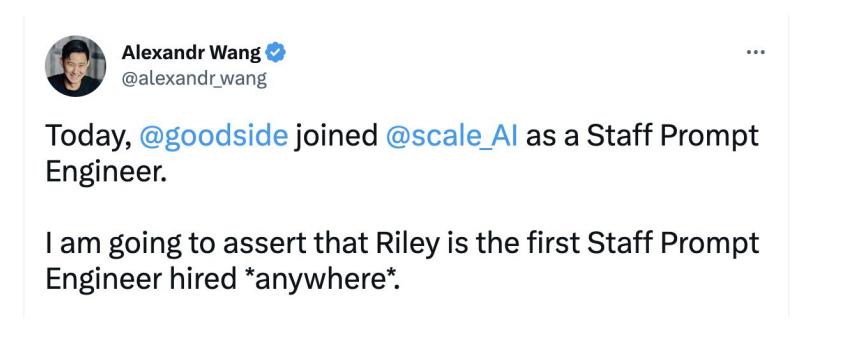
\includegraphics[width=0.8\linewidth,keepaspectratio]{promptengg5}

{\tiny (Ref: Prompt Engineering Sudalai Rajkumar)}

\end{center}		
		


\end{frame}

%%%%%%%%%%%%%%%%%%%%%%%%%%%%%%%%%%%%%%%%%%%%%%%%%%%%%%%%%%%

\begin{frame}[fragile]\frametitle{Read on to learn how to engineer good prompts!}

\begin{itemize}
\item Shin, T., Razeghi, Y., Logan IV, R. L., Wallace, E., \& Singh, S. (2020). AutoPrompt: Eliciting Knowledge from Language Models with Automatically Generated Prompts. Proceedings of the 2020 Conference on Empirical Methods in Natural Language Processing (EMNLP). https://doi.org/10.18653/v1/2020.emnlp-main.346 
\item Kojima, T., Gu, S. S., Reid, M., Matsuo, Y., \& Iwasawa, Y. (2022). Large Language Models are Zero-Shot Reasoners. 
\item Liu, P., Yuan, W., Fu, J., Jiang, Z., Hayashi, H., \& Neubig, G. (2022). Pre-train, Prompt, and Predict: A Systematic Survey of Prompting Methods in Natural Language Processing. ACM Computing Surveys. https://doi.org/10.1145/3560815 
\item Brown, T. B., Mann, B., Ryder, N., Subbiah, M., Kaplan, J., Dhariwal, P., Neelakantan, A., Shyam, P., Sastry, G., Askell, A., Agarwal, S., Herbert-Voss, A., Krueger, G., Henighan, T., Child, R., Ramesh, A., Ziegler, D. M., Wu, J., Winter, C., … Amodei, D. (2020). Language Models are Few-Shot Learners. 
\item Zhao, T. Z., Wallace, E., Feng, S., Klein, D., \& Singh, S. (2021). Calibrate Before Use: Improving Few-Shot Performance of Language Models.
\end{itemize}
\end{frame}



%%%%%%%%%%%%%%%%%%%%%%%%%%%%%%%%%%%%%%%%%%%%%%%%%%%%%%%%%%%
\begin{frame}[fragile]\frametitle{My Sketchnote}

\begin{center}
\includegraphics[width=0.45\linewidth,keepaspectratio]{PromptEng_Sketchnote_Medium}

{\tiny (Ref: https://medium.com/technology-hits/prompting-is-all-you-need-5dddb82bd022)}
\end{center}		

\end{frame}

%%%%%%%%%%%%%%%%%%%%%%%%%%%%%%%%%%%%%%%%%%%%%%%%%%%%%%%%%%%

\begin{frame}[fragile]\frametitle{Take Aways}

Prompt Engineering is an Iterative Process:

\begin{itemize}
\item Try something
\item Analyze where the results do not match the expectations
\item Clarify instructions, gives examples, specify output format, specify constraints, etc
\item Test on a batch of known results.
\end{itemize}
\end{frame}


%%%%%%%%%%%%%%%%%%%%%%%%%%%%%%%%%%%%%%%%%%%%%%%%%%%%%%%%%%%%%%%%%%%%%%%%%%%%%%%%%%
\begin{frame}[fragile]\frametitle{Resources}
\begin{itemize}
\item Prompt Engineering Guide https://github.com/dair-ai/Prompt-Engineering-Guide
\item Awesome ChatGPT Prompts https://github.com/f/awesome-chatgpt-prompts/
\item ChatGPT Prompt Engineering for Developers - Deep Learning AI
\item Learn Prompting https://learnprompting.org/docs/intro
\end{itemize}	 
\end{frame}

